\documentclass[a4paper]{scrbook}
\usepackage{kotex}
\usepackage[colorlinks=true,linkcolor=blue,urlcolor=black,bookmarksopen=true]{hyperref}
\usepackage{caption}
\usepackage{graphicx}
\graphicspath{{./figures}}
\usepackage{bookmark}

\begin{document}
\title{Grasshopper for Fabrication}
\author{Heejin Chae}
\frontmatter
\maketitle
\chapter{Abstract}
\tableofcontents

\mainmatter
\chapter{Introduction}
파라메트릭 모델링(parametric modeling)이란 모델링이력을 그대로 유지하면서 입력 파라미터만 변경해 설계를 자동화(design automation) 하는 방법을 뜻합니다\cite{CHANG2015125}. 
쉽게말해 모델링 시퀀스(sequence)를 만들어 놓은 다음, 입력 파라미터만 변경해 다양한 결과를 탐색할 수 있는 방법 정도로 이해하시면 됩니다. 이와 같은 파라메트릭 모델링은 CATIA, AutoCad 등 여러 소프트웨어 쓰이는 방법입니다. \\
Procedural modeling은 모델링은 위에서 언급한 파라메트릭 모델링을 가능하게 만들기 위해, 모델링 과정을 추상화(abstract)해서 기능으로 만들고 기능들을 서로 논리적으로 연결한 형태를 뜻합니다. 건축분야에서는 McNeel사의 Rhino에 포함되어 있는 Grasshopper\footnote{https://www.grasshopper3d.com/} Revit에 포함된 Dynamo\footnote{https://dynamobim.org/} 등이 있습니다. 이 책에서는 Grasshopper를 대상으로 강의를 진행하고자 합니다. 그 이유는 Dynamo를 이용해 IFC(Industry Foundation Classes)기반 모델링을 수행할 수 있지만, IFC가 모든 문제를 해결해 줄 수 있는 도구가 아니기 떄문에, 실제 사례 중 Rhino와 Grasshopper를 이용해 문제를 해결해야 하는 경우들도 발생합니다. 더군다나 Rhino는 NURBs(Non-univor rational B-spline)기반으로 이루어져, 비정형을 잘 다룰 수 있는 프로그램이기 때문에 박스같이 생긴 정형 형태 뿐만 아니라 곡면이 많은 비정형 형태에 대한 모델링도 수월하게 진행할 수 있습니다. 실제로 Zaha hadid가 설계한 건물인 Morpheus Hotel 디자인을 실제 제작 가능하게 만들기 위해 Revit이 아닌 Rhino + Grasshopper가 쓰인 사례도 존재합니다.\\
dd
\\
dd
\\
dd
\\

\noindent
\begin{minipage}{\textwidth}
    \begin{center}
    \begin{minipage}{0.45\textwidth}
    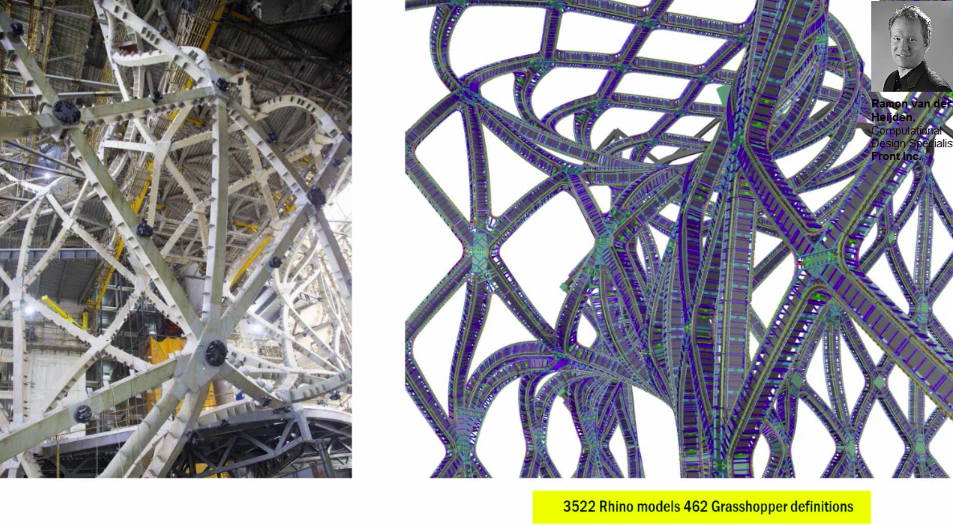
\includegraphics[width=\linewidth]{morpheus_rhToFab}
    \captionof*{figure}{(a) Rhino + Grasshopper를 이용해 만든 모델과 실제 결과물}
    \end{minipage}\hfill
    \begin{minipage}{0.45\textwidth}
    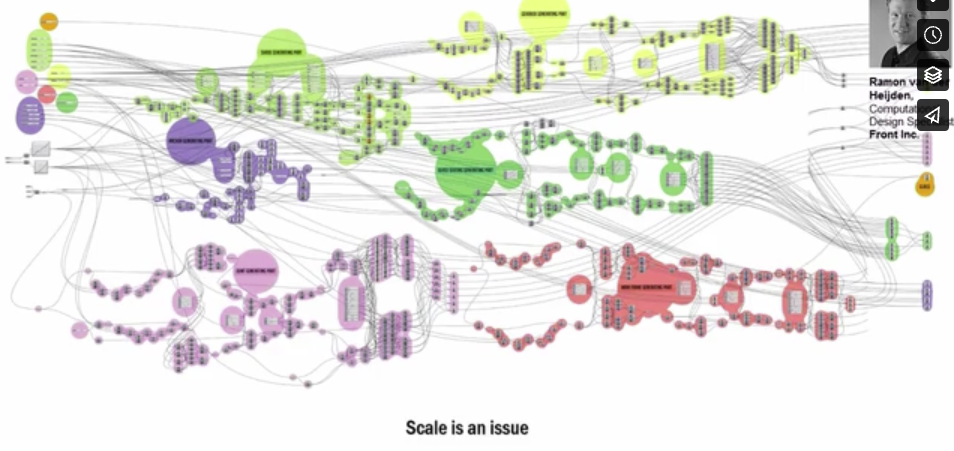
\includegraphics[width=\linewidth]{morpheus_gh} 
    \captionof*{figure}{Morpehus 호텔 프로젝트에 쓰인 Grasshopper 스크립트 일부}   
    \end{minipage}
    \captionof{figure}{Total caption }
    \label{name_label}
    \end{center}
 \end{minipage}
\section{gh}
야호 신난다!! \\
dddd
\\
dddd\\
ddddddfdf\\
\subsection{hello}
신난다다다다!!
\chapter{hi}
Some text ...

\bibliographystyle{plain}
\bibliography{bibliography.bib}
\end{document}